\documentclass[12pt]{article}

\usepackage{graphicx}% Include figure files
\usepackage{dcolumn}% Align table columns on decimal point

% Use Arial font %
\usepackage{helvet}
\renewcommand{\familydefault}{\sfdefault} 

% Default margins and paper properties %
\usepackage[a4, portrait, margin=0.6in]{geometry}

\begin{document}
	\title{Hypothesis plots summary} % Force line breaks with \\
	\author{1666957, Gustavo Espinal Lugo}
	\date{\today} % It is always \today, today, %  but any date may be explicitly specified

	\maketitle
	%\tableofcontents
	
	\section*{Plots and corresponding metadata}
	Number of data points used: 99999,\\
mean expected W mass: 80.36010913 $[GeV/c^{2}]$,\\
mean hypothesis masses $[GeV/c^{2}]$: [<generator object <genexpr> at 0x7fd921c1e510>],\\
mass width: 2.07041274 $[GeV/c^{2}]$,\\
chi\_square value of hypothesis fit: 24.799391035191867\\
	Absolute path to figure: /home/physics/phuxdp/Desktop/PX402 Physics Project/WBosonProject/noQED/plots/muPT\_80.36010913\_2.07041274\_between\_75\_and\_85.png\\
	Next lines are the data of the shown histograms (if needed): \\
	All quantities: 	99999, 80.36010913, [75. 76. 77. 78. 79. 80. 81. 82. 83. 84. 85.], 2.07041274, 24.799391035191867\\
	X\_energ\_vls = [30.1, 30.299999999999997, 30.5, 30.700000000000003, 30.9, 31.1, 31.299999999999997, 31.5, 31.700000000000003, 31.9, 32.1, 32.3, 32.5, 32.7, 32.9, 33.1, 33.3, 33.5, 33.7, 33.9, 34.1, 34.3, 34.5, 34.7, 34.9, 35.1, 35.3, 35.5, 35.7, 35.9, 36.1, 36.3, 36.5, 36.7, 36.9, 37.1, 37.3, 37.5, 37.7, 37.9, 38.1, 38.3, 38.5, 38.7, 38.9, 39.1, 39.3, 39.5, 39.7, 39.9, 40.1, 40.3, 40.5, 40.7, 40.9, 41.1, 41.3, 41.5, 41.7, 41.9, 42.1, 42.3, 42.5, 42.7, 42.9, 43.1, 43.3, 43.5, 43.7, 43.9, 44.1, 44.3, 44.5, 44.7, 44.9, 45.1, 45.3, 45.5, 45.7, 45.9, 46.1, 46.300000000000004, 46.5, 46.7, 46.9, 47.1, 47.300000000000004, 47.5, 47.7, 47.9, 48.1, 48.300000000000004, 48.5, 48.7, 48.9, 49.1, 49.300000000000004, 49.5, 49.7, 49.9]\\
	Y\_data\_bin\_cnts = [266.0, 281.0, 301.0, 304.0, 281.0, 321.0, 336.0, 324.0, 300.0, 328.0, 328.0, 325.0, 318.0, 337.0, 328.0, 371.0, 345.0, 331.0, 383.0, 356.0, 327.0, 345.0, 368.0, 354.0, 369.0, 369.0, 367.0, 344.0, 389.0, 342.0, 384.0, 374.0, 371.0, 385.0, 365.0, 370.0, 364.0, 348.0, 351.0, 340.0, 420.0, 408.0, 389.0, 399.0, 403.0, 398.0, 377.0, 376.0, 348.0, 319.0, 320.0, 307.0, 319.0, 305.0, 286.0, 320.0, 272.0, 260.0, 239.0, 235.0, 228.0, 215.0, 216.0, 211.0, 204.0, 180.0, 196.0, 185.0, 158.0, 154.0, 148.0, 127.0, 134.0, 128.0, 120.0, 120.0, 123.0, 101.0, 104.0, 94.0, 110.0, 105.0, 81.0, 79.0, 100.0, 86.0, 75.0, 76.0, 86.0, 83.0, 80.0, 77.0, 65.0, 70.0, 73.0, 61.0, 64.0, 56.0, 57.0, 66.0]\\
	Y\_model\_bin\_cnts = [293.3139953613281, 274.1718444824219, 262.20001220703125, 241.51925659179688, 193.4226531982422, 162.5618133544922, 277.00787353515625, 245.69247436523438, 254.20297241210938, 267.9975280761719, 211.09300231933594, 227.857177734375, 259.8022155761719, 283.4286804199219, 254.59088134765625, 308.4375, 252.73126220703125, 298.1304626464844, 263.37548828125, 335.0636291503906, 245.20236206054688, 362.4482727050781, 242.3725128173828, 279.9010314941406, 332.10614013671875, 361.15399169921875, 298.3258972167969, 310.101806640625, 314.5876770019531, 245.3587646484375, 334.7698974609375, 247.1780548095703, 350.6287536621094, 455.5913391113281, 334.4283752441406, 408.01275634765625, 207.66851806640625, 268.766845703125, 351.3895568847656, 263.83709716796875, 281.9131164550781, 265.7825622558594, 458.6277160644531, 352.024658203125, 355.4730224609375, 351.4425048828125, 420.45294189453125, 311.5937194824219, 369.5477600097656, 383.499755859375, 306.82989501953125, 301.08123779296875, 358.1631774902344, 234.47679138183594, 301.1171569824219, 429.43792724609375, 275.97802734375, 174.06138610839844, 306.531005859375, 398.5980224609375, 319.2603759765625, 271.90191650390625, 297.3476867675781, 277.53814697265625, 223.22650146484375, 279.4494934082031, 235.9373779296875, 391.8341369628906, 253.5877227783203, 191.29762268066406, 184.3111572265625, 293.7781677246094, 172.0095977783203, 157.24725341796875, 185.24815368652344, 142.16165161132812, 143.38143920898438, 108.30340576171875, 159.6011505126953, 126.0030746459961, 75.29916381835938, 68.94642639160156, 94.34751892089844, 134.1646270751953, 71.9146957397461, 105.8006362915039, 115.0446548461914, 165.56478881835938, 121.86521911621094, 126.58450317382812, 88.50223541259766, 32.55303192138672, 112.40155792236328, 120.7403793334961, 121.25996398925781, 116.5124740600586, 90.07770538330078, 149.0967254638672, 55.78200149536133, 75.59307861328125]\\

    Found optimal massses ($\chi^2$ roots): [80.34443039] $[GeV/c^{2}]$\\
    Uncertainty [GeV/c^2]: 2.842170943040401e-14\\

	\begin{figure}[tb]
		\centering
		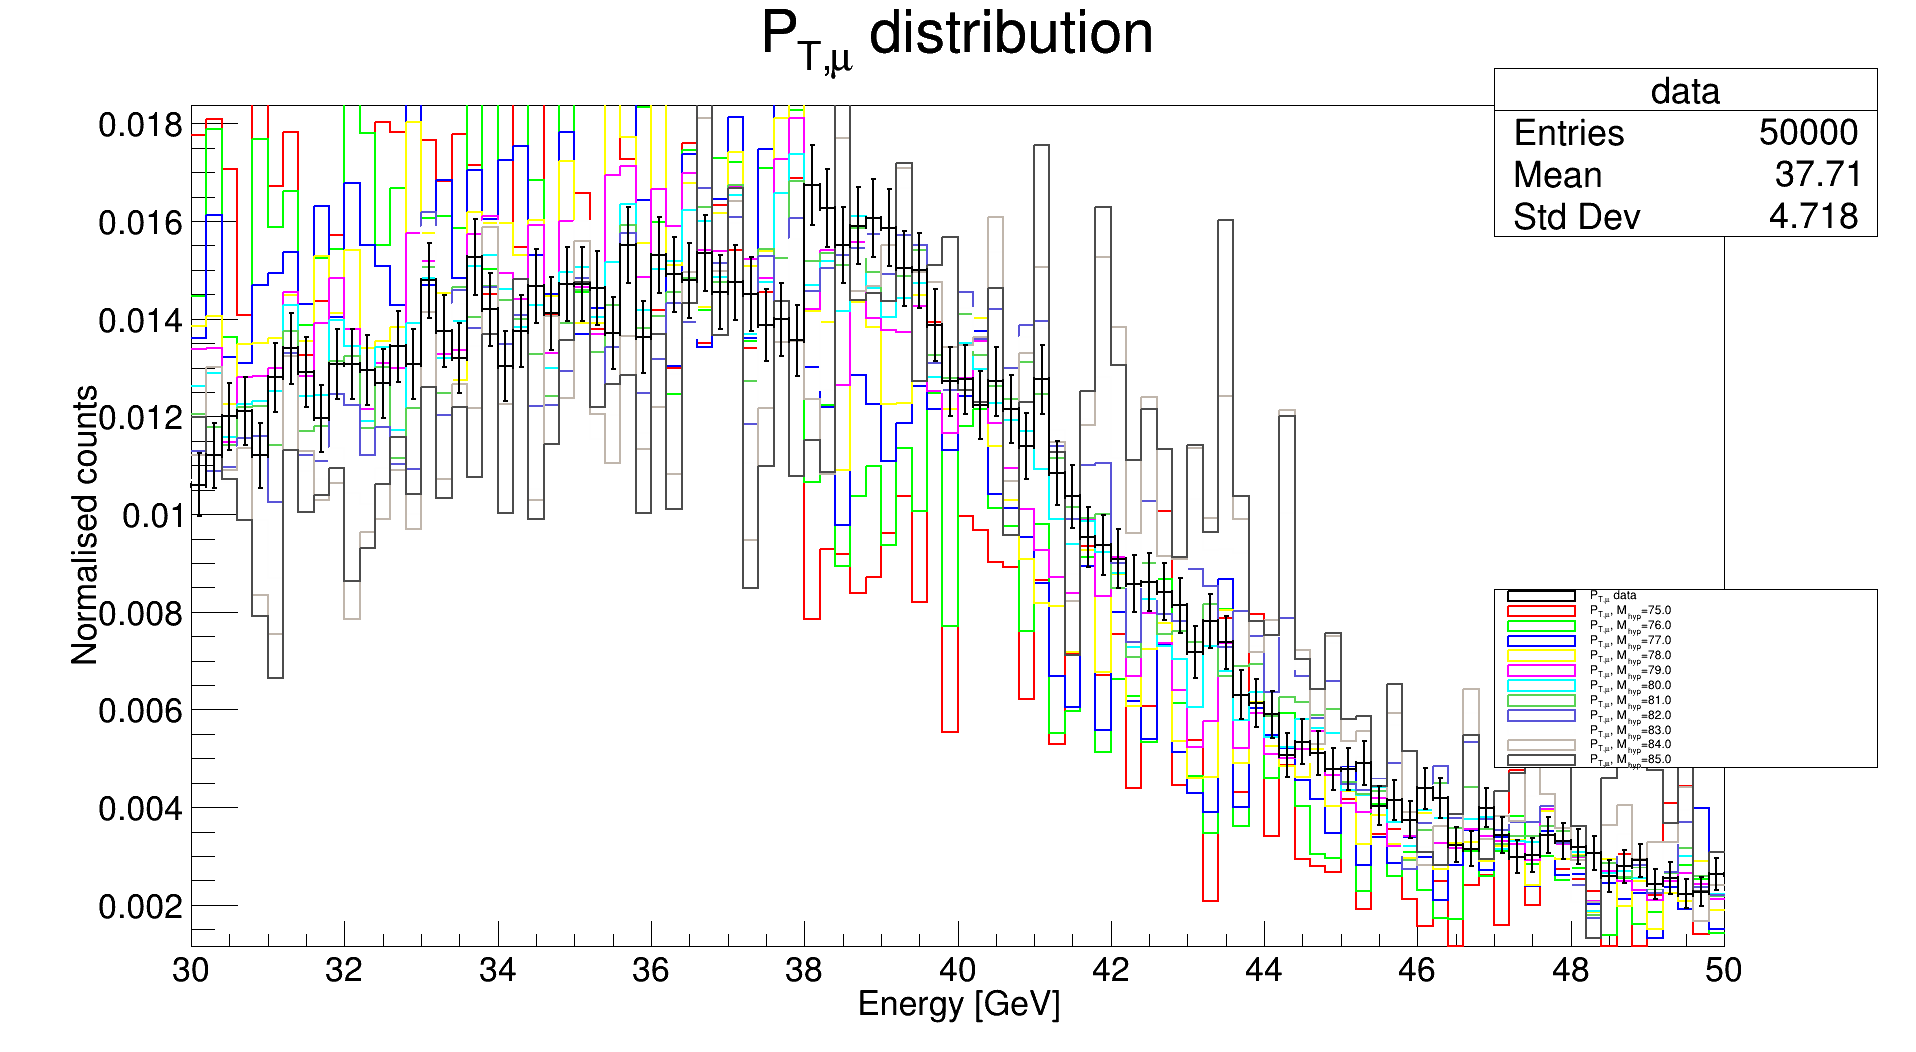
\includegraphics[width=\columnwidth]{/home/physics/phuxdp/Desktop/PX402 Physics Project/WBosonProject/noQED/plots/muPT_80.36010913_2.07041274_between_75_and_85.png}
		\caption{\small Hypothesis masses Number of data points used: 99999,\\
mean expected W mass: 80.36010913 $[GeV/c^{2}]$,\\
mean hypothesis masses $[GeV/c^{2}]$: [<generator object <genexpr> at 0x7fd921c1e510>],\\
mass width: 2.07041274 $[GeV/c^{2}]$,\\
chi_square value of hypothesis fit: 24.799391035191867. }
		\label{fig: fig_0}
	\end{figure}
    Notes: \\
    1) Using mu\_born\_PT as pseudodata and  Mu\_Pt as model/hypothesis\\
    2) Using full run mode\\
       \begin{figure}[tb]
		\centering
		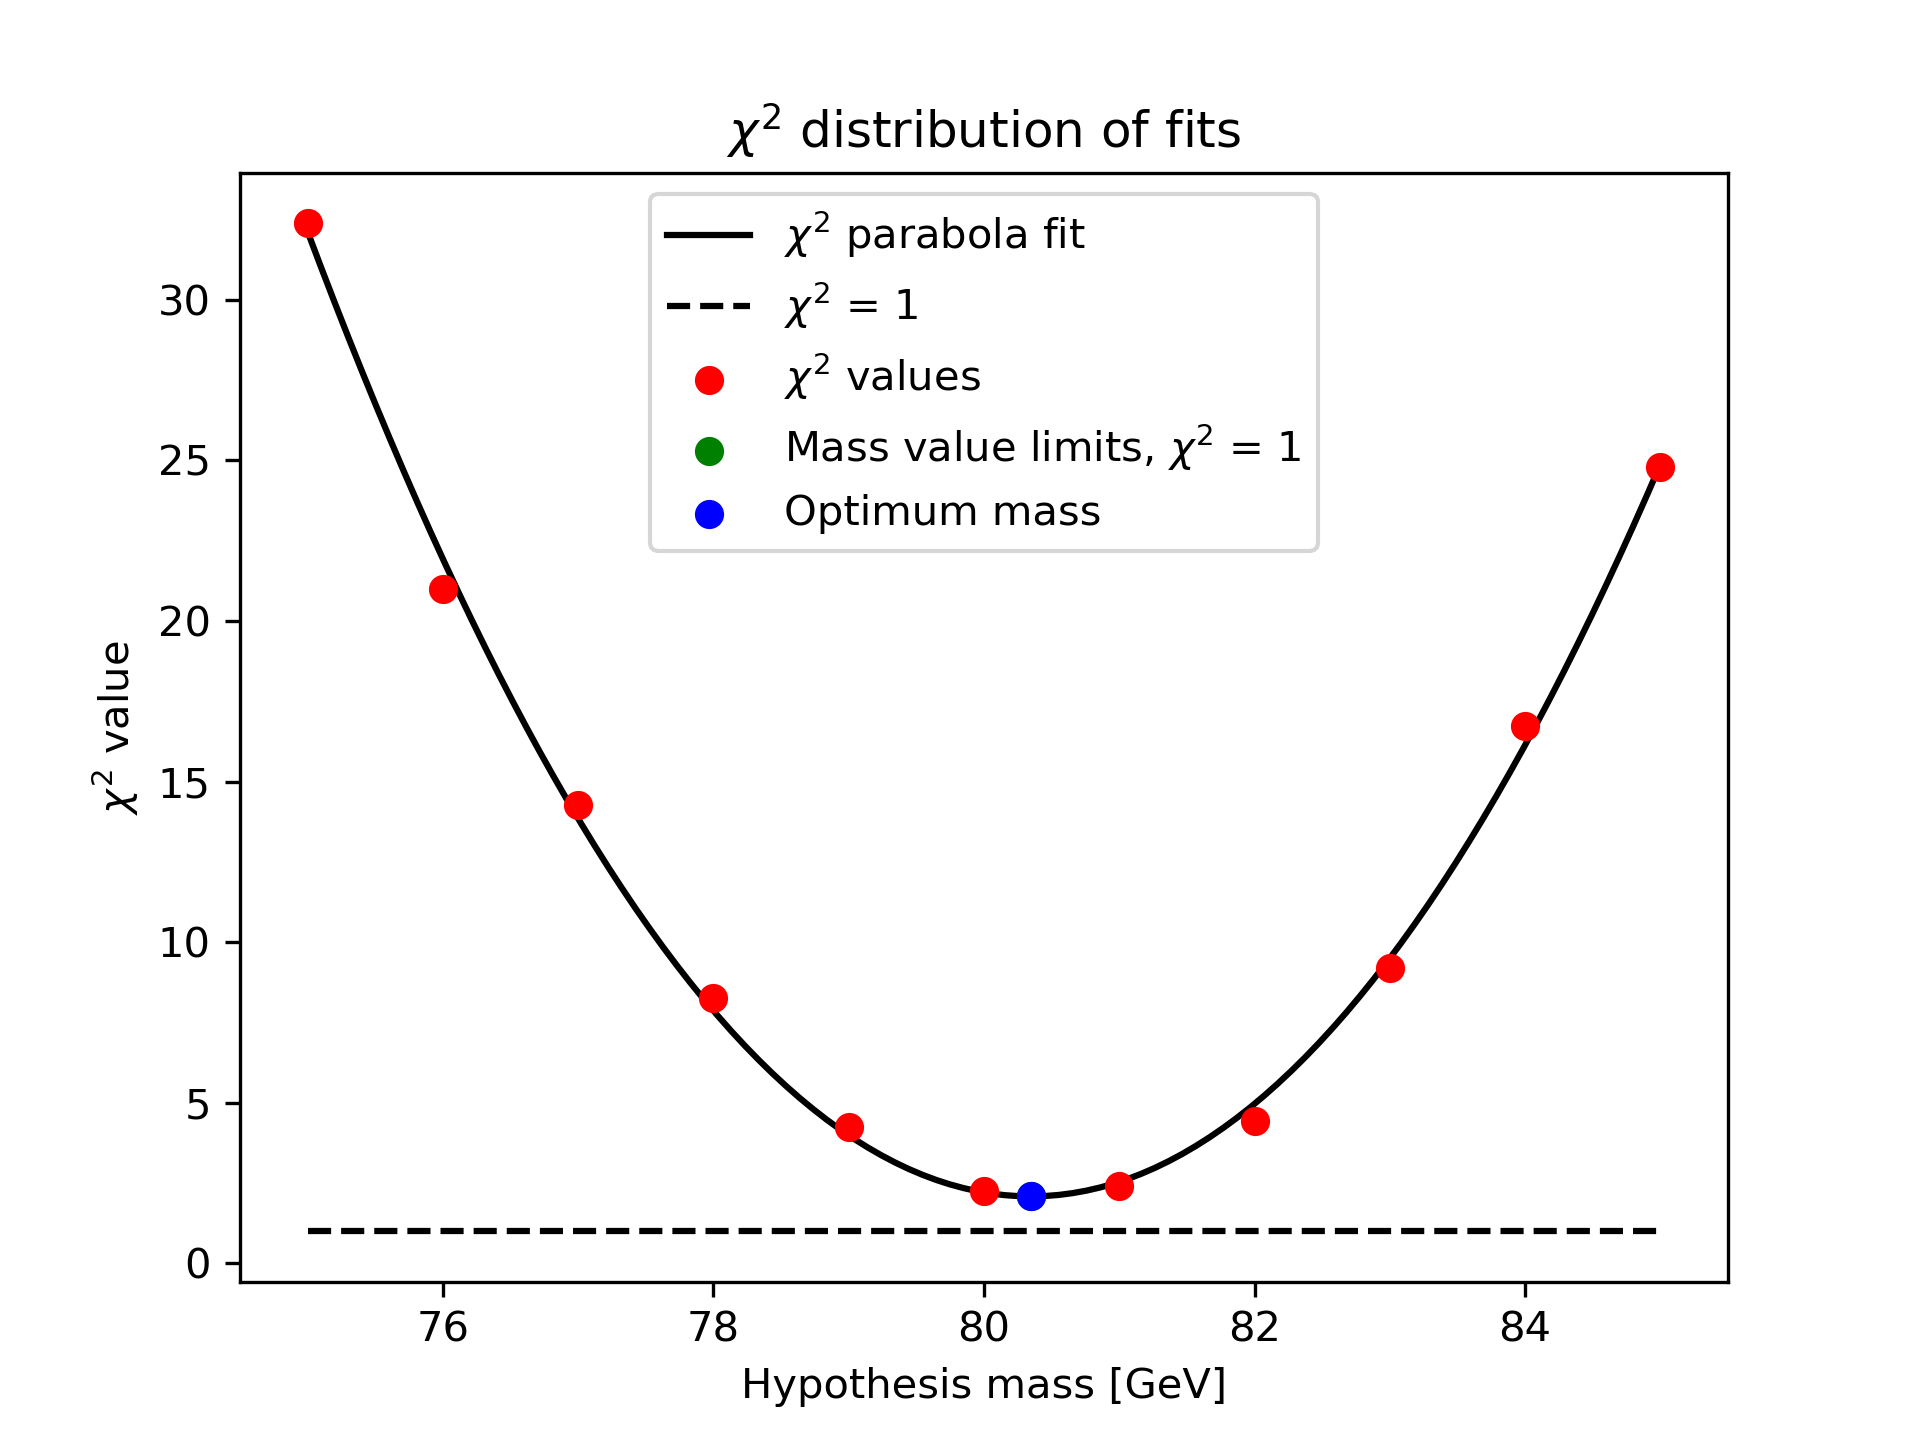
\includegraphics[width=\columnwidth]{/home/physics/phuxdp/Desktop/PX402 Physics Project/WBosonProject/noQED/plots/chi_square_fits_muPT_80.36010913_2.07041274_between_75_and_85.png}
		\caption{\small $\chi^2$ of hypothesis masses. }
		\label{fig: fig_chi_square}
	\end{figure}

    \begin{figure}[tb]
		\centering
		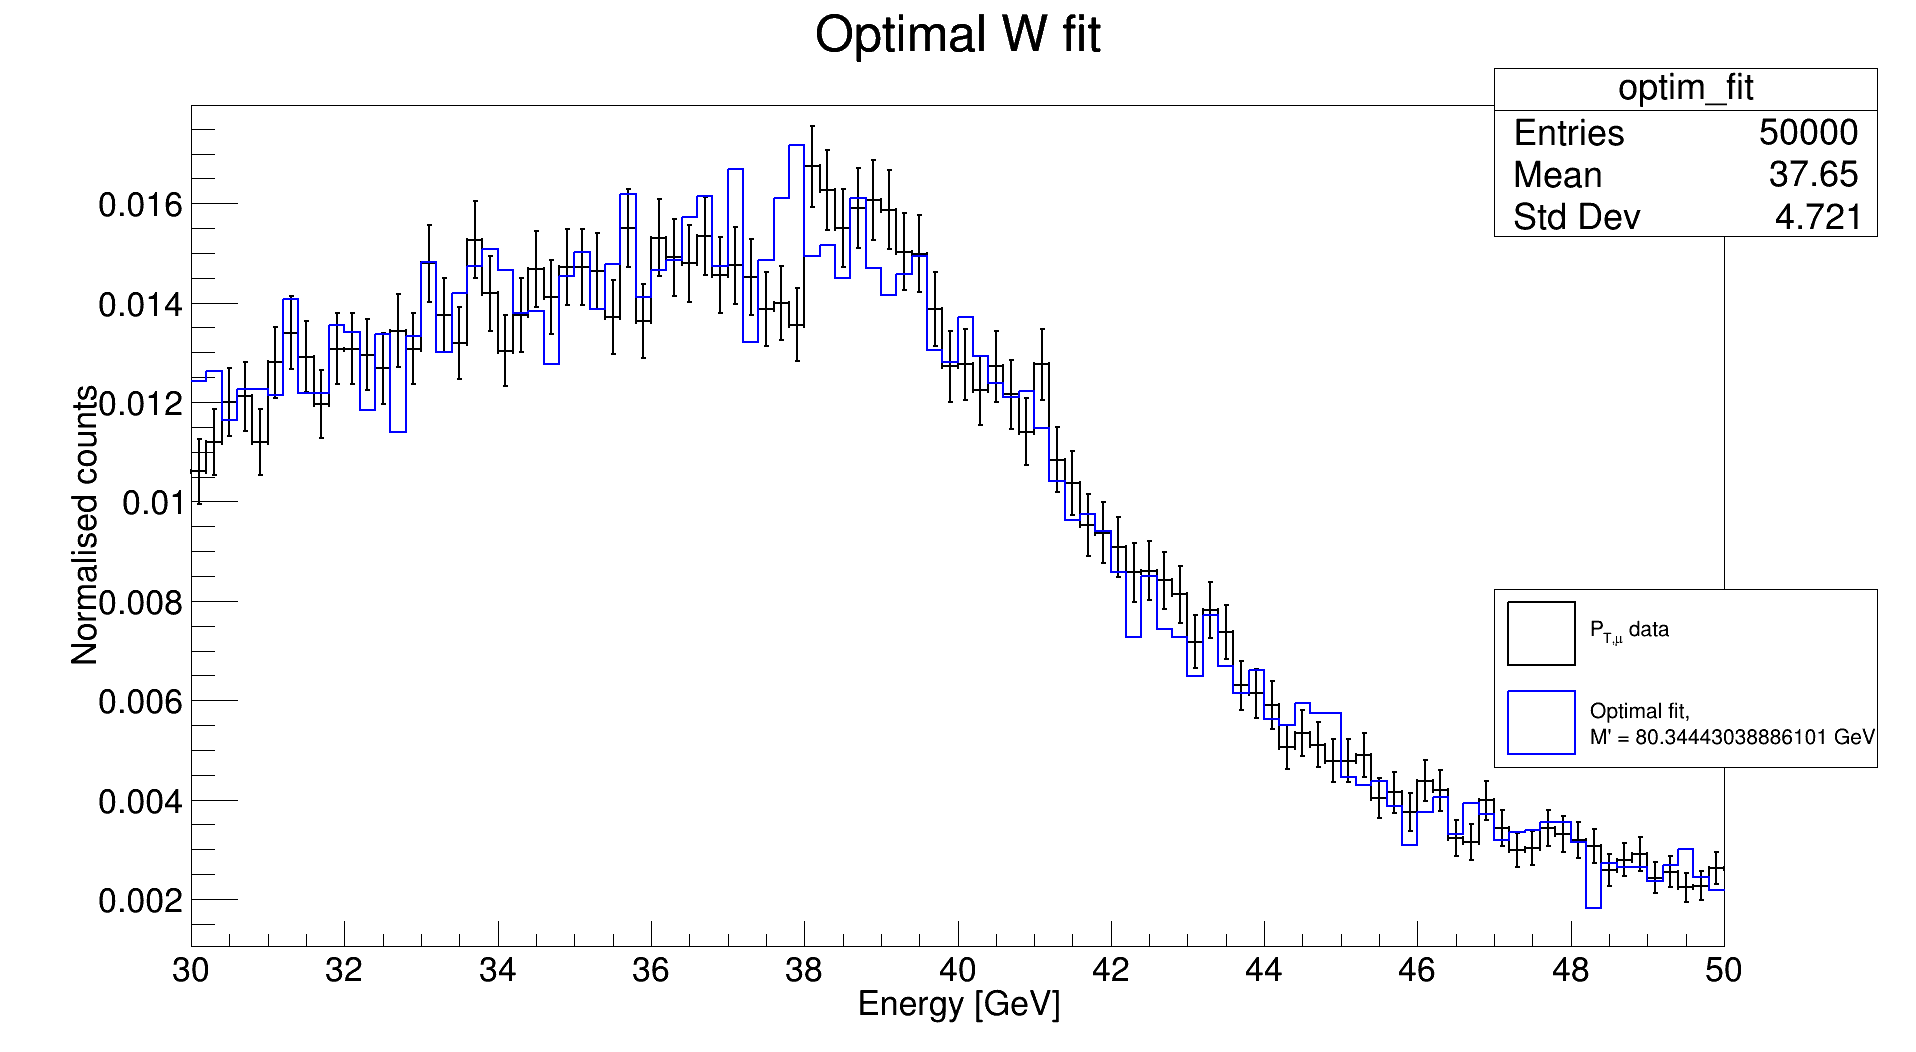
\includegraphics[width=\columnwidth]{/home/physics/phuxdp/Desktop/PX402 Physics Project/WBosonProject/noQED/plots/optimum_muPT_80.36010913_2.07041274_between_75_and_85.png}
		\caption{\small Data and optimum fit with $\chi^2 = 2.081750492423454$. Used the hypothesis mass of 80.34443038886101 $[GeV/c^{2}]$. }
		\label{fig: fig_optim_parms}
	\end{figure}
    
\end{document}